\documentclass[./main.tex]{subfiles}
\begin{document}
\ifSubfilesClassLoaded{\mainmatter}{}

\chapter{Decomposition via \textit{d}-splits} \label{chap:p2c2}

Let $\, d : \XX \to \R \,$ be a symmetric function.

\begin{notation}
    $uv \defeq d(u,v) \,, \quad \forall\, u,v \in X$
\end{notation}
In the following we will implicitly refer to $d$.

\begin{definition}[isolation index]
    Let $A,B$ be non-empty subset of $X$. \\
    Then for every $a,a^\prime \in A$ and $b,b^\prime \in B$ we define
    \[ \beta_{\{a,a^\prime\},\{b,b^\prime\}} \defeq \frac{1}{2}\, \Bigl( \max {\{ ab + a^\prime b^\prime,\, a^\prime b + ab^\prime,\, aa^\prime + bb^\prime \}} - aa^\prime - bb^\prime \,\Bigr) \]
    \[ \aAB \defeq \min_{\substack{a,a^\prime \in A \\ b,b^\prime \in B}}{\beta_{\{a,a^\prime\},\{b,b^\prime\}}} \]
    We call $\aAB = \aAB^d$ the \textbf{isolation index} with respect to $d$.
\end{definition}

\begin{remark}
    We have $\, \beta_{\{a,a^\prime\},\{b,b^\prime\}} \geq 0 \,$ for every $a,a^\prime \in A,\, b,b^\prime \in B$, \\[2pt]
    \bsp since we are subtracting a term that is inside the maximum:
    \[ \max {\{ ab + a^\prime b^\prime,\, a^\prime b + ab^\prime,\, aa^\prime + bb^\prime \}}\ \geq\ aa^\prime + bb^\prime \]
    It follows that also $\, \aAB \geq 0 \,$.
    
    Moreover if $\, \beta_{\{a,a^\prime\},\{b,b^\prime\}} = 0$ \underline{for some} $a,a^\prime \in A,\, b,b^\prime \in B$, \\[2pt]
    \bsp then also $\aAB = 0$.
\end{remark}

\clearpage

\begin{remark}
    If $A$ and $B$ intersect, then $\, \aAB = 0 \,$.
    
    In fact, let $\, x \in A \cap B \,$. Then
    \begin{align*}
        \beta_{\{x\},\{x\}} &= \frac{1}{2}\, \Bigl( \max {\{ xx + xx,\, xx + xx,\, xx + xx \}} - xx - xx \Bigr) \\
        &= \frac{1}{2}\, (xx + xx - xx - xx) = 0
    \end{align*}
    and so $\, \aAB = 0 \,$.
\end{remark}

\begin{proposition} \label{prop:aeqb}
    If $d$ is a pseudo-metric, then for every $t,u,v,w \in X$
    \[ \alpha_{\{t,u\},\{v,w\}} = \beta_{\{t,u\},\{v,w\}} \nospblw \]
\end{proposition}
\begin{proof}
    By (reverse) triangle inequality and the fact that $d$ vanishes on the diagonal, we observe that
    \begin{align*}
        \beta_{\{t\},\{v,w\}} &= \frac{1}{2}\, \Bigl( \max {\{ tv + tw,\, tv + tw,\, \cancel{tt} + vw \}} - \cancel{tt} - vw \Bigr) \\
        &= \frac{1}{2}\, (tv + tw - vw) \\
        &\leq \frac{1}{2}\, (tv + tv) \\
        &= \frac{1}{2}\, \Bigl( \max {\{ tv + tv,\, tv + tv,\, \cancel{tt} + \cancel{vv} \}} - \cancel{tt} - \cancel{vv} \Bigr) \\
        &= \beta_{\{t\},\{v\}}
    \end{align*}
    where we used $\, tv + tw \geq vw \,$ in the first line \\
    \bsp and $\, tw - vw \leq tv \,$ in the second one.

    With analogous calculations we get
    \begin{alignat*}{4}
        &\beta_{\{t\},\{v,w\}} &{}\leq{}& \beta_{\{t\},\{v\}} \,&,& \qquad \beta_{\{t\},\{v,w\}} &{}\leq{}& \beta_{\{t\},\{w\}} \\
        &\beta_{\{u\},\{v,w\}} &{}\leq{}& \beta_{\{u\},\{v\}} \,&,& \qquad \beta_{\{u\},\{v,w\}} &{}\leq{}& \beta_{\{u\},\{w\}} \\
        &\beta_{\{t,u\},\{v\}} &{}\leq{}& \beta_{\{t\},\{v\}} \,&,& \qquad \beta_{\{t,u\},\{v\}} &{}\leq{}& \beta_{\{u\},\{v\}} \\
        &\beta_{\{t,u\},\{w\}} &{}\leq{}& \beta_{\{t\},\{w\}} \,&,& \qquad \beta_{\{t,u\},\{w\}} &{}\leq{}& \beta_{\{u\},\{w\}}
    \end{alignat*}

    Again by (reverse) triangle inequality
    \begin{alignat*}{4}
        tv + uw - tu -vw &\,\leq\, tv &{}+{}& tw &{}-{}& vw &\,{}={}\,& 2\beta_{\{t\},\{v,w\}} \\
        &\,\leq\, uv &{}+{}& uw &{}-{}& vw &\,{}={}\,& 2\beta_{\{u\},\{v,w\}} \\
        &\,\leq\, tv &{}+{}& uv &{}-{}& tu &\,{}={}\,& 2\beta_{\{t,u\},\{v\}} \\
        &\,\leq\, tw &{}+{}& uw &{}-{}& tu &\,{}={}\,& 2\beta_{\{t,u\},\{w\}} \\
        uv + tw - tu - vw &\,\leq\, tv &{}+{}& tw &{}-{}& vw &\,{}={}\,& 2\beta_{\{t\},\{v,w\}} \\
        &\,\leq\, uv &{}+{}& uw &{}-{}& vw &\,{}={}\,& 2\beta_{\{u\},\{v,w\}} \\
        &\,\leq\, tv &{}+{}& uv &{}-{}& tu &\,{}={}\,& 2\beta_{\{t,u\},\{v\}} \\
        &\,\leq\, tw &{}+{}& uw &{}-{}& tu &\,{}={}\,& 2\beta_{\{t,u\},\{w\}}
    \end{alignat*}

    Since
    \[ \beta_{\{t,u\},\{v,w\}} = \frac{1}{2}\, \Bigl( \max {\{ tv + uw,\, uv + tw,\, tu + vw \}} - tu - vw \Bigr) \]
    we have proven that $\beta_{\{t,u\},\{v,w\}}$ is smaller than \\[2pt]
    \bsp all other possible $\beta$ indices for the quartet $\bigl\{ \{t,u\},\{v,w\} \bigr\}$. \medskip

    This implies by definition of the isolation index
    \[ \alpha_{\{t,u\},\{v,w\}} = \beta_{\{t,u\},\{v,w\}} \nospblw \]
\end{proof}

\begin{corollary} \label{cor:aeqa}
    If $d$ is a pseudo-metric and $\, \min {\{ \card{A},\card{B} \}} \geq 2 \,$ \\[2pt]
    \bsp (that is both A and B have at least 2 elements), then
    \[ \aAB = \alpha_{\{a,a^\prime\},\{b,b^\prime\}} \]
    for some $\, a \neq a^\prime \in A \,$ and $\, b \neq b^\prime \in B \,$.
\end{corollary}
\begin{proof}
    Let $\bigl\{ \{a,a^\prime\},\{b,b^\prime\} \bigr\}$ be the quartet that minimizes the $\beta$ index.
    
    Then, for the previous inequalities about $\beta$ indices \\
    \bsp and the hypothesis on the number of elements of $A$ and $B$, \\
    we conclude that $\, a \neq a^\prime \,$ and $\, b \neq b^\prime \,$.
    
    Using the previous \autoref{prop:aeqb}
    \[ \aAB = \beta_{\{a,a^\prime\},\{b,b^\prime\}} = \alpha_{\{a,a^\prime\},\{b,b^\prime\}} \nospblw \qedhere \]
\end{proof}

\begin{definition}[splits and $d$-splits]
    A \textbf{partial split} (of $X$) is an unordered pair $\{A,B\}$ with $A,B \subseteq X$. \\
    A \textbf{(total) split} (of $X$) is partial split $\{A,B\}$ such that $A \cup B = X$.
    
    A partial/total \textbf{$\bm{d}$-split} is a partial/total split $\{A,B\}$ such that $\aAB^d > 0$. \\
    Notice that in this case $A$ and $B$ must be disjoint. \bigskip
    
    The sets $A$ and $B$ are called \textbf{parts} of the split. \\
    We call a split \textbf{trivial} if one of the parts contains only one element. \\
    A partial split of the form $\bigl\{ \{a,a^\prime\}, \{b,b^\prime\} \bigr\}$ is called \textbf{quartet}.

    We denote the set of all splits of $X$ with $\Sc(X)$ \\
    \bsp and the set of all $d$-splits of $X$ with $\Sc_d(X)$.
\end{definition}

\begin{definition}[$d$-convex set]
    A set $S \subseteq X$ is \textbf{$\bm{d}$-convex} if
    \[ \forall\, x,y \in S,\ \forall\, z \in X, \qquad xz + zy = xy \implies z \in S \]
\end{definition}

\begin{proposition}
    If $\{A,B\}$ is a $d$-split, then $A$ and $B$ are $d$-convex.
\end{proposition}
\begin{proof}
    Let $x,y \in A$ and $z \in X$ such that $xz + zy = xy$.
    
    Since $X = A \cup B$, we have $z \in A$ or $z \in B$.
    
    If by absurd $z \in B$, then
    \begin{align*}
        \beta_{\{x,y\},\{z\}} &= \frac{1}{2}\, \Bigl( \max {\{ xz + yz,\, xz + yz,\, xy + \cancel{zz} \}} - xy - \cancel{zz} \Bigr) \\
        &= \frac{1}{2}\, (xz + yz - xy) = \frac{1}{2}\, (xy - xy) = 0
    \end{align*}
    that implies $\aAB = 0$. \absurd

    Then it must be $z \in A$ and so $A$ is $d$-convex.
\end{proof}

\clearpage

\begin{definition}[extension of $d$-splits]
    We say that a partial $d$-split $\{A,B\}$ \textbf{extends} another partial $d$-split $\{A^\prime,B^\prime\}$ \\[2pt]
    \bsp if $A \supseteq A^\prime$ and $B \supseteq B^\prime$ (or $A \supseteq B^\prime$ and $B \supseteq A^\prime$). \\[2pt]
    We denote it $\{A,B\} \succcurlyeq \{A^\prime,B^\prime\}$.
    
    Notice that $\, \aAB \leq \alpha_{A^\prime,B^\prime} \,$ (it’s a minimum on a larger set).
\end{definition}

\begin{lemma} \label{lemma:teo1}
    Let $\{A,B\}$ be a partial $d$-split.
    
    Then for every $\, a_1,a_2 \in A,\ b_1,b_2 \in B,\ x \in X \setminus (A \cup B) \,$
    \[ \alpha_{\{a_1,a_2,x\},\{b_1,b_2\}} \,+\, \alpha_{\{a_1,a_2\},\{b_1,b_2,x\}} \,\leq\, \beta_{\{a_1,a_2\},\{b_1,b_2\}} \]
\end{lemma}
\begin{proof}
    Suppose by absurd that exist $\, a_1,a_2,\ b_1,b_2,\, x \,$ such that
    \[ \alpha_{\{a_1,a_2,x\},\{b_1,b_2\}} \,+\, \alpha_{\{a_1,a_2\},\{b_1,b_2,x\}} \,>\, \beta_{\{a_1,a_2\},\{b_1,b_2\}} \]

    Observe that $\beta_{\{a_1,a_2\},\{b_1,b_2\}} > 0$ since $\{A,B\}$ is a partial $d$-split, so also
    \[ \alpha_{\{a_1,a_2,x\},\{b_1,b_2\}} > 0 \,, \qquad \alpha_{\{a_1,a_2\},\{b_1,b_2,x\}} > 0 \]
    because isolation indices are not negative.

    From this, and by definition of isolation index, we have
    \begin{alignat*}{2}
        \beta_{\{a_1,x\},\{b_1,b_2\}} &\geq \alpha_{\{a_1,a_2,x\},\{b_1,b_2\}} &{}>{}& 0 \\
        \beta_{\{a_1,a_2\},\{x,b_i\}} &\geq \alpha_{\{a_1,a_2\},\{b_1,b_2,x\}} &{}>{}& 0 \,, \quad i = 1,2
    \end{alignat*} \smallskip
    
    Let $\{i,j\} = \{1,2\}$ so that 
    \[ \beta_{\{a_1,x\},\{b_1,b_2\}} = \frac{1}{2}\, \bigl(\, a_1 b_j + x b_i - a_1 x - b_1 b_2 \,\bigr) \]
    in fact, since $\beta_{\{a_1,x\},\{b_1,b_2\}} > 0$, the maximum
    \[ \max {\{ a_1 b_1 + x b_2,\, a_1 b_2 + x b_1,\, a_1 x + b_1 b_2 \}} \eqspace{2pt}{0pt} \]
    cannot be $a_1 x + b_1 b_2$.
    
    For the same reason we have
    \begin{align*}
        \beta_{\{a_1,a_2\},\{x,b_i\}} &= \frac{1}{2}\, \Bigl( \max {\{ a_1 x + a_2 b_i,\, a_1 b_i + a_2 x \}} - a_1 a_2 - x b_i \Bigr) \\
        \beta_{\{a_1,a_2\},\{b_1,b_2\}} &= \frac{1}{2}\, \Bigl( \max {\{ a_1 b_1 + a_2 b_2,\, a_1 b_2 + a_2 b_1 \}} - a_1 a_2 - b_1 b_2 \Bigr)
    \end{align*} \medskip
    
    From the previous inequalities we have
    \begin{multline*}
        \beta_{\{a_1,x\},\{b_1,b_2\}} + \beta_{\{a_1,a_2\},\{x,b_i\}} \geq \\[2pt]
        \geq \alpha_{\{a_1,a_2,x\},\{b_1,b_2\}} + \alpha_{\{a_1,a_2\},\{b_1,b_2,x\}} > \beta_{\{a_1,a_2\},\{b_1,b_2\}}
    \end{multline*} 
    and by substituting the expressions for the $\beta$ indices
    \begin{gather*}
        \begin{multlined}[\linewidth-\multlinegap]
            \frac{1}{2}\, \Bigl( a_1 b_j + \cancel{x b_i} - a_1 x - \cancel{b_1 b_2} \\[-5pt]
            + \max {\{ a_1 x + a_2 b_i,\, a_1 b_i + a_2 x \}} - a_1 a_2 - \cancel{x b_i} \Bigr) >
        \end{multlined} \\
        > \frac{1}{2}\, \Bigl( \max {\{ a_1 b_1 + a_2 b_2,\, a_1 b_2 + a_2 b_1 \}} - a_1 a_2 - \cancel{b_1 b_2} \Bigr)
    \end{gather*}
    simplifying we obtain
    \begin{align*}
        a_1 b_j - a_1 x {}+{}& \max {\{ a_1 x + a_2 b_i,\, a_1 b_i + a_2 x \}} \\
        {}>{}& \max {\{ a_1 b_1 + a_2 b_2,\, a_1 b_2 + a_2 b_1 \}}
    \end{align*}
    
    If by absurd $\, \max {\{ a_1 x + a_2 b_i,\, a_1 b_i + a_2 x \}} = a_1 x + a_2 b_i \,$, \\[2pt]
    the previous inequality would become
    \[ a_1 b_j - \cancel{a_1 x} + \cancel{a_1 x} + a_2 b_i > \max {\{ a_1 b_1 + a_2 b_2,\, a_1 b_2 + a_2 b_1 \}} \]
    but since $a_1 b_j + a_2 b_i$ is a term of the maximum on the right, \\
    this is a contradiction. \absurd
    
    So we must have $\, a_1 x + a_2 b_i < a_1 b_i + a_2 x \,$ and thus
    \begin{align*}
        a_1 b_1 + a_1 b_2 - a_1 x + a_2 x &= a_1 b_j - a_1 x + a_1 b_i + a_2 x \\
        &> \max {\{ a_1 b_1 + a_2 b_2,\, a_1 b_2 + a_2 b_1 \}}
    \end{align*}
    
    For this to be true we need
    \[ a_1 b_k + a_2 x > a_1 x + a_2 b_k\,, \quad k = 1,2 \]
    By symmetry, interchanging $a_1$ and $a_2$ (notice that we can do this because the absurd hypothesis is symmetrical in $a_1,a_2$), \\
    \bsp we obtain the other strict inequality. \absurd \qedhere
\end{proof}

In the following theorem we use the notation
\[ \sum \bigl\{\, a \mathrel{\big|} \dots \bigr\}\ \defeq\ \sum_{\cdots} a \nospblw \] \vspace{-\baselineskip}

\begin{theorem}[{\cites[Theorem 1]{BD92a}}] \label{teo:teo1}
    Let $\{A_0,B_0\}$ be a partial $d$-split. Then
    \[ \mathlarger{\sum} \Bigl\{\, \aAB \mathrel{\Big|} \{A,B\} \in \Sc(X) \,,\ \{A,B\} \succcurlyeq \{A_0,B_0\} \Bigr\} \,\leq\, \alpha_{A_0,B_0} \nospblw \]
\end{theorem}
\begin{proof}
    Let $a_1,a_2 \in A_0$ and $b_1,b_2 \in B_0$ such that 
    \[ \alpha_{A_0,B_0} = \beta_{\{a_1,a_2\},\{b_1,b_2\}} \nospblw \]
    
    From the previous \autoref{lemma:teo1}, we have for every $\, x \in X \setminus (A_0 \cup B_0)$
    \begin{align*}
        \alpha_{A_0 \cup \{x\},\, B_0} + \alpha_{A_0,\, B_0 \cup \{x\}} &\leq \alpha_{\{a_1,a_2,x\},\{b_1,b_2\}} + \alpha_{\{a_1,a_2\},\{b_1,b_2,x\}} \\
        &\mathcolor{blue}{\leq} \beta_{\{a_1,a_2\},\{b_1,b_2\}} \\
        &= \alpha_{A_0,B_0}
    \end{align*}
    
    This also proves the theorem in the case $\, \card{X \setminus (A_0 \cup B_0)} = 1 \,$. \bigskip
    
    We prove the general case by induction on $\, \card{X \setminus (A_0 \cup B_0)} \,$.
    
    We have already seen the base case.
    
    Let $\, \card{X \setminus (A_0 \cup B_0)} = n > 1 \,$ and $x \in X \setminus (A_0 \cup B_0) \,$.

    \begin{spacing}{1.1}
    Observe that the $d$-splits extending $\{A_0,B_0\}$ are exactly the collection of those extending $\bigl\{ A_0 \cup \{x\}, B_0 \bigr\}$ and those extending $\bigl\{ A_0, B_0 \cup \{x\} \bigr\}$. \\[2pt]
    In fact, since $d$-splits are partitions, if $\{A,B\}$ extends $\{A_0,B_0\}$ \\
    -- say WLOG $\, A \supseteq A_0 \,$ and $\, B \supseteq B_0 \,$ -- it must be $x \in A$ or $x \in B$; \\
    that is $\, A \supseteq A_0 \cup \{x\} \,$ or $\, B \supseteq B_0 \cup \{x\} \,$.
    \end{spacing}

    Moreover, \vspace{-5pt}
    \begin{align*}
        \card{\, X \setminus \bigl( (A_0 \cup \{x\}) \cup B_0 \bigr) \,} &= n-1 \\[5pt]
        \card{\, X \setminus \bigl( A_0 \cup (B_0 \cup \{x\}) \bigr) \,} &= n-1
    \end{align*}

    So we can apply the inductive step:
    \begin{gather*}
        \mathlarger{\sum} \Bigl\{\, \aAB \mathrel{\Big|} \{A,B\} \in \Sc(X) \,,\ \{A,B\} \succcurlyeq \{A_0,B_0\} \Bigr\} = \\
        \begin{split}
            = &\mathlarger{\sum} \Bigl\{\, \aAB \mathrel{\Big|} \{A,B\} \in \Sc(X) \,,\ \{A,B\} \succcurlyeq \bigl\{ A_0 \cup \{x\}, B_0 \bigr\} \Bigr\} \\
            &\mathlarger{\sum} \Bigl\{\, \aAB \mathrel{\Big|} \{A,B\} \in \Sc(X) \,,\ \{A,B\} \succcurlyeq \bigl\{ A_0, B_0 \cup \{x\} \bigr\} \Bigr\} \mathcolor{red}{\leq}
        \end{split} \\
        \mathcolor{red}{\leq}\, \alpha_{A_0 \cup \{x\},\, B_0} + \alpha_{A_0,\, B_0 \cup \{x\}} \,\leq\, \alpha_{A_0,B_0}
    \end{gather*}
    where the last inequality is the one proved at the beginning.
\end{proof}

\begin{remark}
    We can substitute splits with $d$-splits in the sum \\
    \bsp (splits that are not $d$-splits do not contribute).
\end{remark}

\begin{remark}
    The proof of \autoref{teo:teo1} tells us that we can build a tree of partial splits inductively by fixing a partial split as the root and adding one element at a time to each part of the partial split, obtaining two children.
    
    In this tree the sum of the isolation indices of the children is less than or equal to the isolation index of the parent. \\[2pt]
    In particular the sum of the isolation indices of all the nodes that share a common ancestor is less than or equal to the isolation index of the common ancestor. \\[2pt]
    As a consequence the sum of the isolation indices of all the nodes at the same level is less than or equal to the isolation index of the root (\autoref{teo:teo1} is just a special case where the level is that of the leaves).

    Observe that such tree is not unique, but depends on the order in which the elements are added. \\
    In particular if $\{A,B\}$ is an extension of $\{A_0,B_0\}$, than it exists an extension tree rooted in $\{A_0,B_0\}$ that contains $\{A,B\}$.
\end{remark}

\clearpage

\begin{figure}[h]
    \centering
    \fbox{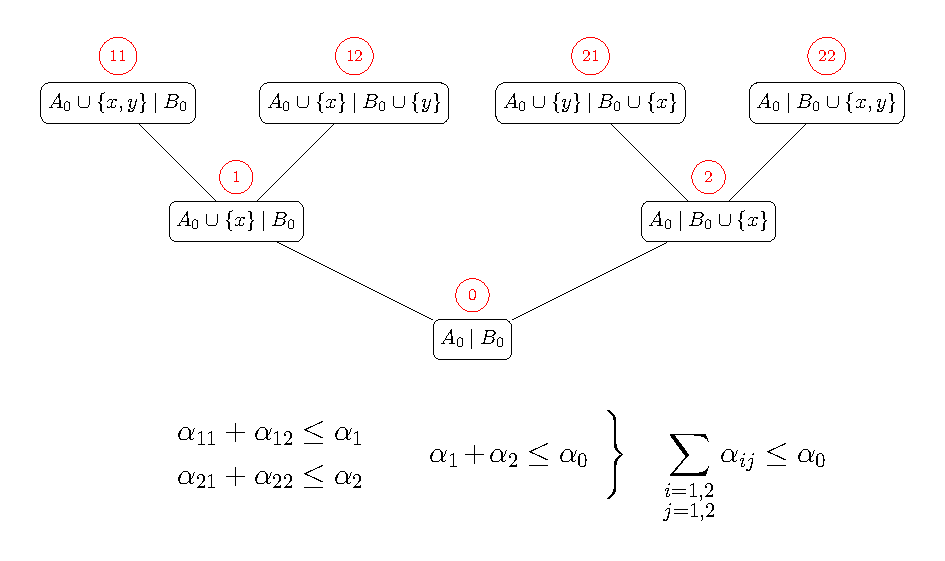
\includegraphics[width=\textwidth]{tikz/split-tree.pdf}}
\end{figure}

\begin{corollary}[{\cites[Corollary 1]{BD92a}}] \label{cor:cor1}
    Let $\{A,B\}$ a $d$-split and let $a_1,a_2 \in A$ and $b_1,b_2 \in B$ such that
    \[ \aAB = \beta_{\{a_1,a_2\},\{b_1,b_2\}} \]
    Then $\{A,B\}$ is the unique $d$-split that extends $\bigl\{ \{a_1,a_2\},\{b_1,b_2\} \bigr\}$.
\end{corollary}
\begin{proof}
    Observe that $\bigl\{ \{a_1,a_2\},\{b_1,b_2\} \bigr\}$ is a partial $d$-split.
    
    In fact, if by absurd
    \[ \alpha_{\{a_1,a_2\},\{b_1,b_2\}} = \beta_{\{a_1,a_2\},\{b_1,b_2\}} = 0 \eqspace{-5pt}{2pt} \]
    then $\aAB = 0$, but $\{A,B\}$ is a $d$-split. \absurd

    By applying \autoref{teo:teo1}
    \begin{align*}
        \aAB &\mathcolor{blue}{\leq} \mathlarger{\sum} \biggl\{\, \alpha_{A^\prime,B^\prime} \mathrel{\bigg|}
            \begin{array}{c}
                \{A^\prime,B^\prime\} \in \Sc_d(X) \,,  \\[2pt]
                 \{A^\prime,B^\prime\} \succcurlyeq \bigl\{ \{a_1,a_2\},\{b_1,b_2\} \bigr\}
            \end{array}
        \biggr\} \\
        &\leq \alpha_{\{a_1,a_2\},\{b_1,b_2\}} \\
        &\leq \beta_{\{a_1,a_2\},\{b_1,b_2\}} = \aAB
    \end{align*}

    Since the sum is equal to $\aAB$ and $\{A,B\}$ is a member of the range of the sum, this means that $\{A,B\}$ is the only $d$-split that extends $\bigl\{ \{a_1,a_2\},\{b_1,b_2\} \bigr\}$.
\end{proof}

\begin{definition}[split metric]
    Given $A,B$ non-empty disjoint subsets of $X$, \\
    \bsp the \textbf{split metric} $\dAB$ on $A \cup B$ is defined as
    \[ \dAB(u,v) \defeq
        \begin{cases}
        \, 0 \,,    & \text{if}\ u,v \in A\ \text{or}\ u,v \in B \\
        \, 1 \,,    & \text{otherwise}
        \end{cases}
    \nospblw \]
\end{definition}
This definition is slightly different from that given previously, \\
\bsp because we do not require $A \cup B = X$ (we now admit \textit{partial} split metrics).

\begin{proposition}
    The split $\{A,B\}$ is the only $\dAB$-split and its isolation index is $1$.
\end{proposition}
\begin{proof}
    In fact, let us consider $\{A,B\}$ and another split $\{A^\prime,B^\prime\}$, \\
    with the following intersections:
    \[ A \cap A^\prime \,,\quad A \cap B^\prime \,,\quad B \cap A^\prime \,,\quad B \cap B^\prime \nospblw \]

    Since $\, A \cup B = A^\prime \cup B^\prime = X \,$ and $\, A,B,A^\prime,B^\prime \neq \emptyset \,$, \\
    at least two of these intersection must be non-empty.
    
    We can divide in cases. \bigskip

    If all the intersections are non-empty, we can pick
    \[ a_1 \in A \cap A^\prime \,,\quad a_2 \in A \cap B^\prime \,,\quad b_1 \in B \cap A^\prime \,,\quad b_2 \in B \cap B^\prime \]
    then, with respect to $\dAB$, we have
    \begin{align*}
        a_1 b_1 + a_2 b_2 &= 1 + 1 = 2 \\
        a_1 b_2 + a_2 b_1 &= 1 + 1 = 2 \\
        a_1 a_2 + b_1 b_2 &= 0 + 0 = 0
    \end{align*}
    \[ \beta_{\{a_1,b_1\},\{a_2,b_2\}} = \frac{1}{2}\, \Biggl( \max {\Biggl\{\!\!
        \begin{array}{c}
            a_1 b_1 + a_2 b_2, \\
            a_1 b_2 + a_2 b_1, \\
            \cancel{a_1 a_2 + b_1 b_2}
        \end{array}
    \!\!\Biggr\}} - a_1 b_1 - a_2 b_2 \Biggr) = 0 \]
    so $\alpha_{A^\prime,B^\prime} = 0$. \bigskip \smallskip

    If only three of the intersections are non-empty \\
    -- say WLOG $A \cap A^\prime \,,\ B \cap A^\prime \,,\ B \cap B^\prime$ -- then we can pick
    \[ a_1 \in A \cap A^\prime \,,\quad b_1 \in B \cap A^\prime \,,\quad b_2 \in B \cap B^\prime \]
    and then, with respect to $\dAB$, we have
    \begin{align*}
        a_1 b_1 + b_2 b_2 &= 1 + 0 = 1 \\
        a_1 b_2 + b_1 b_2 &= 1 + 0 = 1
    \end{align*}
    \[ \beta_{\{a_1,b_1\},\{b_2\}} = \frac{1}{2}\, \biggl( \max {\biggl\{\!\!
        \begin{array}{c}
            a_1 b_2 + b_1 b_2, \\
            a_1 b_1 + b_2 b_2
        \end{array}
    \!\!\biggr\}} - a_1 b_1 - b_2 b_2 \biggr) = 0 \]
    so $\alpha_{A^\prime,B^\prime} = 0$. \bigskip \smallskip

    If only two intersections are non-empty, then $\{A,B\} = \{A^\prime,B^\prime\}$.
    
    In fact, say WLOG $\, A \cap B^\prime,\, B \cap A^\prime = \emptyset \,$. \\
    Since $\, A \cup B = X \,$, then we have $A^\prime \subseteq A$ and $B^\prime \subseteq B$. \\
    But since $\, A^\prime \cup B^\prime = X \,$, we also have $A \subseteq A^\prime$ and $B \subseteq B^\prime$, \\
    \bsp so it must be $A^\prime = A$ and $B^\prime = B$.
    
    Now \underline{for every} $a_1,a_2 \in A$ and $b_1,b_2 \in B$, with respect to $\dAB$,
    \begin{align*}
        a_1 b_1 + a_2 b_2 &= 1 + 1 = 2 \\
        a_1 b_2 + a_2 b_1 &= 1 + 1 = 2 \\
        a_1 a_2 + b_1 b_2 &= 0 + 0 = 0
    \end{align*}
    \[ \beta_{\{a_1,a_2\},\{b_1,b_2\}} = \frac{1}{2}\, \Biggl( \max {\Biggl\{\!\!
        \begin{array}{c}
            a_1 b_1 + a_2 b_2, \\
            a_1 b_2 + a_2 b_1, \\
            \cancel{a_1 a_2 + b_1 b_2}
        \end{array}
    \!\!\Biggr\}} - \cancel{a_1 a_2 - b_1 b_2} \Biggr) = 1 \]
    so $\alpha_{A,B} = 1$.
\end{proof}

\clearpage

\begin{definition}[split-prime function]
    A function $\, d : \XX \to \R \,$ is \textbf{split-prime} if it does not admit any $d$-split.
    \[ \Sc_d(X) = \emptyset \nospblw \]
\end{definition}

\begin{definition}[dissimilarity function]
    A function $\, d : \XX \to \R \,$ is a \textbf{dissimilarity function} if
    \begin{itemize}
        \item $d(x,y) = d(y,x) \,,$  \tabto*{10em} $\forall\, x,y \in X$
        \item $d(x,x) = 0 \,,$       \tabto*{10em} $\forall\, x \in X$
        \item $d(x,y) \geq 0 \,,$    \tabto*{10em} $\forall\, x,y \in X$
    \end{itemize}
\end{definition}
In practice, it is a pseudo-metric without triangle inequality.

\begin{theorem}[{\cites[Theorem 2]{BD92a}}] \label{teo:teo2}
    Let $\, d : \XX \to \R \,$ be a symmetric function. \\
    Let $\lambda_S \in \R$ such that $\lambda_S \leq \alpha_S^d$ if $S$ is a $d$-split \\
    \phantom{Let $\lambda_S \in \R$ such } and $\lambda_S = 0$\ \ \ otherwise.

    Then
    \[ \dpr \ \defeq\  d \ -\! \sum_{S \,\in\, \Sc(X)} \lambda_S \cdot \delta_S \eqspace{-2pt}{-5pt} \]
    is a symmetric function such that
    \[ \alpha_S^\dpr = \alpha_S^d - \lambda_S \,, \quad \forall\, S \in \Sc(X) \eqspace{2pt}{0pt} \]

    In addition, if $d$ is a dissimilarity function (or a pseudo-metric), \\
    then $\dpr$ is also a dissimilarity function (or a pseudo-metric).
\end{theorem}
\begin{proof}
    It suffices to prove the assertions for
    \[ \dpr = \widetilde{d} \defeq d - \lambda \cdot \delta_{A_0,B_0} \]
    where $\{A_0,B_0\}$ is a $d$-split and $\, \lambda \leq \alpha_{A_0,B_0}^d \,$.

    Then the general case follows by subtracting one split metric at a time (formally induction on the number of non-zero $\lambda$’s). \bigskip

    We use the following notation: $\ uv = d(u,v),\ \ \forall\, u,v \in X$
    \[ \alpha = \alpha^d \,,\ \ \beta = \beta^d, \qquad \widetilde{\alpha} = \alpha^{\widetilde{d}} \,,\ \ \widetilde{\beta} = \beta^{\widetilde{d}} \nospblw \] \bigskip

    Clearly $\widetilde{d}$ is a symmetric function (since $d$ and $\delta$ are such).

    For every $u,v \in X$ we have
    \[ \widetilde{d}(u,v) = \bigg\{
        \begin{array}{cl}
            uv \,,              & \quad \text{if}\ \{u,v\} \subseteq A_0\ \text{or}\ \{u,v\} \subseteq B_0 \\
            uv - \lambda \,,    & \quad \text{otherwise}
        \end{array} 
    \] \bigskip

    Suppose that $d$ is a dissimilarity function.

    Then $\, \widetilde{d}(u,u) = d(u,u) = 0 \,$. For $u \in A_0$ and $v \in B_0$ we have
    \[ \lambda \leq \alpha_{A_0,B_0} \leq \beta_{\{u\},\{v\}} = uv \]
    thus $\, \widetilde{d}(u,v) = uv - \lambda \geq 0 \,$, so $\widetilde{d}$ is a dissimilarity function. \bigskip

    Now suppose that $d$ is a pseudo-metric. \\
    We have to verify the triangle inequality for $\widetilde{d}$.
    
    Let $u,v,w \in X$. If they all belong to $A_0$ or all to $B_0$, \\
    \bsp then $d$ and $\widetilde{d}$ agrees on $\{u,v,w\}$ and we are done. \\[2pt]
    Otherwise, say WLOG $\, u,v \in A_0$ and $w \in B_0$, then we get
    \begin{align*}
        \lambda \leq \alpha_{A_0,B_0} &\leq \beta_{\{u,v\},\{w\}} \\
        &= \frac{1}{2}\, \Bigl( \max {\{ uw + vw,\, uv + \cancel{ww} \}} - uv - \cancel{ww} \Bigr) \\
        &= \frac{1}{2}\, (uw + vw - uv)
    \end{align*}
    where we used the triangle inequality for $d$, and by rearranging
    \[ \underbrace{uv}_{\widetilde{d}(u,v)}\ \leq\ \underbrace{(uw - \lambda)}_{\widetilde{d}(u,w)} \,+\, \underbrace{(vw - \lambda)}_{\widetilde{d}(v,w)} \]

    \hrulefill \clearpage

    For the remainder of the proof $d$ is just a symmetric function. \bigskip \bigskip

    Let $\, \{t,u\},\{v,w\} \subseteq X \,$. \\[5pt]
    We claim that
    \[ \widetilde{\beta}_{\{t,u\},\{v,w\}} = \bigg\{
        \begin{array}{cl}
            \beta_{\{t,u\},\{v,w\}} - \lambda \,,   & \quad \text{if}\ \{A_0,B_0\} \succcurlyeq \bigl\{ \{t,u\},\{v,w\} \bigr\} \\[2pt]
            \beta_{\{t,u\},\{v,w\}} \,,             & \quad \text{otherwise}
        \end{array}
    \] \bigskip

    Suppose $\, \{A_0,B_0\} \succcurlyeq \bigl\{ \{t,u\},\{v,w\} \bigr\} \,$.
    
    Since $\{A_0,B_0\}$ is a $d$-split, the $\max$ get simplified
    \[ \beta_{\{t,u\},\{v,w\}} = \frac{1}{2}\, \Bigl( \max {\{ tv + uw,\, tw + uv \}} - tu - vw \Bigr) > 0 \]
    and we get the following inequalities
    \begin{gather*}
        \lambda \,\leq\, \alpha_{A_0,B_0} \,\leq\, \beta_{\{t,u\},\{v,w\}} \\[2pt]
        2 \lambda \,\leq\, \max {\biggl\{\!\!
            \begin{array}{c}
                tv + uw \\
                tw + uv
            \end{array}
        \!\!\biggr\}} - tu - vw \\[2pt]
        tu + vw \,\leq\, \max {\biggl\{\!\!
            \begin{array}{c}
                (tv - \lambda) + (uw - \lambda) \\
                (tw - \lambda) + (uv - \lambda)
            \end{array}
        \!\!\biggr\}}
    \end{gather*}
    from which
    \begin{align*}
        \widetilde{\beta}_{\{t,u\},\{v,w\}} &= \frac{1}{2}\, \Biggl( \max {\Biggl\{\!
            \begin{array}{c}
                \tilde{d}(t,v) + \tilde{d}(u,w) \\
                \tilde{d}(t,w) + \tilde{d}(u,v) \\
                \tilde{d}(t,u) + \tilde{d}(v,w)
            \end{array}
        \!\!\Biggr\}} - \tilde{d}(t,u) - \tilde{d}(v,w) \Biggr) \\
        &= \frac{1}{2}\, \Biggl( \max {\Biggl\{\!\!
            \begin{array}{c}
                (tv - \lambda) + (uw - \lambda) \\
                (tw - \lambda) + (uv - \lambda) \\
                tu + vw
            \end{array}
        \!\!\Biggr\}} - tu - vw \Biggr) \\
        &= \frac{1}{2}\, \biggl( \max {\biggl\{\!\!
            \begin{array}{c}
                tv + uw \\
                tw + uv
            \end{array}
        \!\!\biggr\}} - 2 \lambda - tu - vw \biggr) \\[2pt]
        &= \beta_{\{t,u\},\{v,w\}} - \lambda
    \end{align*}

\clearpage

    Suppose instead that WLOG $\, t,v \in A_0$ and $u,w \in B_0$.
    
    Since $\{A_0,B_0\}$ is a $d$-split, the $\max$ get simplified
    \begin{align*}
        \beta_{\{t,v\},\{u,w\}} &= \frac{1}{2}\, \Bigl( \max {\{ tu + vw,\, tw + vu \}} - tv - uw \Bigr) \\
        &\geq\, \alpha_{A_0,B_0} \,\geq\, \lambda
    \end{align*}
    from which, similarly as before, we get the inequality
    \[ tv + uw \leq \max {\{ tu + vw - 2 \lambda,\, tw + uv - 2 \lambda \}} \]
    from which
    \begin{align*}
        \widetilde{\beta}_{\{t,u\},\{v,w\}} &= \frac{1}{2}\, \Biggl( \max {\Biggl\{\!\!
            \begin{array}{c}
                tv + uw \\
                (tw - \lambda) + (uv - \lambda) \\
                (tu - \lambda) + (vw - \lambda)
            \end{array}
        \!\!\Biggr\}} - (tu - \lambda) - (vw - \lambda) \Biggr) \\
        &= \frac{1}{2}\, \biggl( \max {\biggl\{\!\!
            \begin{array}{c}
                tw + uv \\
                tu + vw \\
            \end{array}
        \!\!\biggr\}} - \cancel{2 \lambda} - tu - vw + \cancel{2 \lambda} \biggr) \\[2pt]
        &= \beta_{\{t,u\},\{v,w\}}
    \end{align*} \medskip

    If instead $A_0$ or $B_0$ contains three of $\, t,u,v,w$ \\
    -- say WLOG $\, t,u,v \in A_0$ and $w \in B_0$ -- then
    \begin{align*}
        \widetilde{\beta}_{\{t,u\},\{v,w\}} &= \frac{1}{2}\, \Biggl( \max {\Biggl\{\!\!
            \begin{array}{c}
                tv + (uw - \lambda) \\
                (tw - \lambda) + uv \\
                tu + (vw - \lambda)
            \end{array}
        \!\!\Biggr\}} - tu - (vw - \lambda) \Biggr) \\
        &= \frac{1}{2}\, \Biggl( \max {\Biggl\{\!\!
            \begin{array}{c}
                tv + uw \\
                tw + uv \\
                tu + vw
            \end{array}
        \!\!\Biggr\}} \ \cancel{-\ \lambda} - tu - (vw \ \cancel{-\ \lambda}) \Biggr) \\[2pt]
        &= \beta_{\{t,u\},\{v,w\}}
    \end{align*} \smallskip

    If instead all of $\, t,u,v,w \,$ are contained in $A_0$ or all in $B_0$, \\
    then $\widetilde{d}$ acts as $d$ on these elements, so
    \[ \widetilde{\beta}_{\{t,u\},\{v,w\}} = \beta_{\{t,u\},\{v,w\}} \]

    \hrulefill \clearpage

    Finally, we claim that for every split $\{A,B\}$
    \[ \widetilde{\alpha}_{A,B} = \bigg\{
        \begin{array}{cl}
            \alpha_{A,B} - \lambda \,,   & \quad \text{if}\ \{A,B\} = \{A_0,B_0\} \\[2pt]
            \alpha_{A,B} \,,             & \quad \text{otherwise}
        \end{array}
    \nospblw \] \bigskip

    Since, as has been proven before, for every $\, t,u \in A_0 \,,\, v,w \in B_0$
    \[ \widetilde{\beta}_{\{t,u\},\{v,w\}} \mathcolor{red}{=} \beta_{\{t,u\},\{v,w\}} - \lambda \]
    then, by taking the minimum, $\ \widetilde{\alpha}_{A_0,B_0} = \alpha_{A_0,B_0} - \lambda \,$. \bigskip \bigskip

    Now suppose $\, \{A,B\} \neq \{A_0,B_0\} \,$.

    We are going to prove the double inequality between $\aAB$ and $\widetilde{\alpha}_{A,B}$. \bigskip \medskip

    Choose $a,a^\prime \in A$ and $b,b^\prime \in B$ such that
    \[ \aAB = \beta_{\{a,a^\prime\},\{b,b^\prime\}} \nospblw \]

    We claim that $\{A_0,B_0\}$ cannot extend $\bigl\{ \{a,a^\prime\},\{b,b^\prime\} \bigr\}$. \medskip
    
    In fact, if by absurd it is an extension, then there are two cases.

    If $\, \aAB = 0 \,$, then $\, \beta_{\{a,a^\prime\},\{b,b^\prime\}} = \aAB = 0 \,$. \\[3pt]
    Since $\, \{A_0,B_0\} \succcurlyeq \bigl\{ \{a,a^\prime\},\{b,b^\prime\} \bigr\} \,$, we have $\, \alpha_{A_0,B_0} = 0 \,$. \\[2pt]
    But $\{A_0,B_0\}$ is a $d$-split. \absurd

    If $\, \aAB > 0 \,$, then $\{A,B\}$ is a $d$-split extending $\bigl\{ \{a,a^\prime\},\{b,b^\prime\} \bigr\}$. \\[2pt]
    But by \autoref{cor:cor1}, such a $d$-split extension is unique, \\[2pt]
    so $\{A,B\} = \{A_0,B_0\}$. \absurd \medskip

    Since we proved that $\, \{A_0,B_0\} \not\succcurlyeq \bigl\{ \{a,a^\prime\},\{b,b^\prime\} \bigr\} \,$, we get
    \[ \aAB = \beta_{\{a,a^\prime\},\{b,b^\prime\}} \mathcolor{red}{=} \widetilde{\beta}_{\{a,a^\prime\},\{b,b^\prime\}} \geq \widetilde{\alpha}_{A,B} \nospblw \] \smallskip

    Now let $t,u \in A$ and $v,w \in B \,$.
    
    If $\{A_0,B_0\}$ does not extend $\bigl\{ \{t,u\},\{v,w\} \bigr\}$, then
    \[ \aAB \leq \beta_{\{t,u\},\{v,w\}} \mathcolor{red}{=} \widetilde{\beta}_{\{t,u\},\{v,w\}} \]

    Otherwise, if $\{A_0,B_0\}$ does extend $\bigl\{ \{t,u\},\{v,w\} \bigr\}$, then
    \begin{align*}
        \lambda &\leq \alpha_{A_0,B_0} \\
        \aAB + \lambda &\leq \alpha_{A_0,B_0} + \aAB
    \end{align*}
    \begin{align*}
        \aAB &\leq (\aAB + \alpha_{A_0,B_0}) - \lambda \\
        &\mathcolor{blue}{\leq} \alpha_{\{t,u\},\{v,w\}} - \lambda \\
        &\leq \beta_{\{t,u\},\{v,w\}} - \lambda \\
        &\mathcolor{red}{=} \widetilde{\beta}_{\{t,u\},\{v,w\}}
    \end{align*}
    where we used \autoref{teo:teo1}, since $\{A,B\}$ and $\{A_0,B_0\}$ are two extensions of $\bigl\{ \{t,u\},\{v,w\} \bigr\}$, which is a partial $d$-split: \\[2pt]
    in fact, if by absurd $\, \alpha_{\{t,u\},\{v,w\}} = 0 \,$, then also $\, \alpha_{A_0,B_0} = 0 \,$. \absurd \bigskip

    Since we proved that for every $\, t,u \in A,\, v,w \in B$ \bigskip
    \begingroup \nospabv \nospblw
    \begin{align*}
        \aAB &\leq \widetilde{\beta}_{\{t,u\},\{v,w\}}
        \intertext{then}
        \aAB &\leq \min \widetilde{\beta}_{\{t,u\},\{v,w\}} = \widetilde{\alpha}_{A,B}
    \end{align*}
    \endgroup
\end{proof}

\begin{corollary}[split decomposition / canonical decomposition]
    For any symmetric function $\, d : \XX \to \R \,$ we can write
    \[ d = d_0 + \sum_{S \,\in\, \Sc(X)} \alpha_S^d \cdot \delta_S \eqspace{2pt}{2pt} \]
    where $d_0$ is a split-prime (symmetric) function.

    We call $d_0$ the \textbf{split-prime residue} of $d$.
\end{corollary}
\begin{proof}
    Apply \autoref{teo:teo2} with $\, \lambda_S = \alpha_S^d,\ \forall\, S \in \Sc_d(X) \,$. Let
    \[ d_0 \defeq d - \sum_{S \,\in\, \Sc(X)} \alpha_S^d \cdot \delta_S \]
    Then, if $S$ is a $d$-split $\, \alpha_S^{d_0} = \alpha_S^d - \lambda_S = \alpha_S^d - \alpha_S^d = 0\, $ \\[2pt]
    otherwise \tabto*{10em} $\, \alpha_S^{d_0} = \alpha_S^d - \lambda_S = 0 - 0 = 0 \,$.
\end{proof}

\begin{remark}
    We can sum over only the $d$-splits, since the others do not contribute (they have zero coefficient).
\end{remark}

\begin{remark}
    The residue of a split-prime function coincides with the function itself (there are no splits on which to decompose).
\end{remark}

\begin{corollary}[{\cites[Corollary 2]{BD92a}}] \label{cor:cor2}
    Suppose $\, d : \XX \to \R \,$ is a pseudo-metric. \\
    Let $\lambda \geq 0$ and $x \in X$. Consider
    \[ \dpr \defeq d + \lambda \cdot \delta_x \nospblw \]

    Then $\dpr$ and $d$ have the same split-prime residue and
    \[ \alpha_S^\dpr = 
        \begin{cases}
        \, \alpha_S^d + \lambda \,, & \text{if}\ S = \bigl\{ \{x\},\, X \setminus \{x\} \bigr\} \\
        \, \alpha_S^d \,,           & \text{otherwise}
        \end{cases}
    \nospblw \]
\end{corollary}
\begin{proof}
    If $\lambda = 0$, then $\dpr = d$, and there is nothing to prove. \\
    So we can assume WLOG that $\lambda > 0$.
    
    Observe that for every $\, u,v \in X \setminus \{x\} \,$ we have
    \begin{align*}
        \beta_{\{x\},\{u,v\}}^\dpr &= \frac{1}{2}\, \biggl( \max {\biggl\{\!\!
            \begin{array}{c}
                (xu + \lambda) + (xv + \lambda) \\
                \cancel{xx} + uv
            \end{array}
        \!\!\biggr\}} - \cancel{xx} - uv \biggr) \\[2pt]
        &= \frac{1}{2}\, (xu + xv + 2 \lambda - uv) \\
        &= \lambda + \frac{1}{2}\, (xu + xv - uv) \geq \lambda
    \end{align*}
    where we used the triangle inequality for $d$.

    Therefore $\, \alpha_{\{x\},\, X \setminus \{x\}}^\dpr \geq \lambda > 0 \,$ and thus $\bigl\{ \{x\},\, X \setminus \{x\} \bigr\}$ is a $\dpr$-split. \\[3pt]
    Since $\, d = \dpr - \lambda \cdot \delta_x \,$, we get the thesis by applying \autoref{teo:teo2} to $\dpr$.

    Moreover, since $\, \alpha_{\{x\},\, X \setminus \{x\}}^\dpr = \alpha_{\{x\},\, X \setminus \{x\}}^d + \lambda \,$
    \begin{align*}
        (\dpr)_0 &= \dpr - \sum{\alpha_S^\dpr \cdot \delta_S} - \alpha_{\{x\},\, X \setminus \{x\}}^\dpr \cdot \delta_x \\
        &= (d + \cancel{\lambda \cdot \delta_x}) - \sum{\alpha_S^d \cdot \delta_S} - \bigl(\, \alpha_{\{x\},\, X \setminus \{x\}}^d \,\cancel{+ \lambda} \,\bigr) \cdot \delta_x = d_0
    \end{align*}
    where the sums range over the splits different from $\bigl\{ \{x\},\, X \setminus \{x\} \bigr\}$. \qedhere
\end{proof}

\begin{proposition} \label{prop:teo2ext}
    In the same hypothesis of \autoref{teo:teo2}, \\ for every \underline{partial} split $T$ we have
    \[ \alpha_T^\dpr = \alpha_T^d - \sum \lambda_S \]
    where the sum ranges over all the (total) splits that extend $T$.
\end{proposition}
\begin{proof}
    We can recycle the proof of \autoref{teo:teo2} with some minor variations. \\
    For brevity the steps that are identical are omitted. \bigskip

    Consider a $d$-split $\{A_0,B_0\}$, $\, \lambda \leq \alpha_{A_0,B_0}^d \,$ and
    \[ \widetilde{d} \defeq d - \lambda \cdot \delta_{A_0,B_0} \]
    We claim that for every \underline{partial} split $\{A,B\}$ we have
    \[ \widetilde{\alpha}_{A,B} = \bigg\{
        \begin{array}{cl}
            \alpha_{A,B} - \lambda \,,   & \quad \text{if}\ \{A_0,B_0\} \succcurlyeq \{A,B\} \\[2pt]
            \alpha_{A,B} \,,             & \quad \text{otherwise}
        \end{array}
    \nospblw \] \bigskip

    Suppose $\, \{A_0,B_0\} \succcurlyeq \{A,B\} \,$.

    We know from the first part of the proof that
    \[ \widetilde{\beta}_{\{t,u\},\{v,w\}} = \bigg\{
        \begin{array}{cl}
            \beta_{\{t,u\},\{v,w\}} - \lambda \,,   & \quad \text{if}\ \{A_0,B_0\} \succcurlyeq \bigl\{ \{t,u\},\{v,w\} \bigr\} \\[2pt]
            \beta_{\{t,u\},\{v,w\}} \,,             & \quad \text{otherwise}
        \end{array}
    \]
    
    For every $\, t,u \in A \,,\, v,w \in B \,$, \\[2pt]
    we have that $\, \{A_0,B_0\} \succcurlyeq \bigl\{ \{t,u\},\{v,w\} \bigr\} \,$, so
    \[ \widetilde{\beta}_{\{t,u\},\{v,w\}} \mathcolor{red}{=} \beta_{\{t,u\},\{v,w\}} - \lambda \]
    Then, by taking the minimum on $A,B$, we have $\ \widetilde{\alpha}_{A,B} = \alpha_{A,B} - \lambda \,$. \bigskip \medskip

    Now suppose $\, \{A_0,B_0\} \not\succcurlyeq \{A,B\} \,$.

    We claim that $\{A_0,B_0\}$ cannot extend the quartet that realizes $\alpha_{A,B}^d$. \medskip

    Suppose by absurd that $\{A_0,B_0\}$ is indeed such an extension.
    
    In order to apply the \autoref{cor:cor1} in the case $\, \aAB > 0 \,$, \\[2pt]
    we need to restrict $\{A_0,B_0\}$ to $A \cup B$.
    
    Since both $\alpha_{A_0,B_0} > 0$ and $\aAB > 0$, \\
    \bsp we have that $A_0,B_0$ and $A,B$ respectively are disjoint; \\
    so we can suppose WLOG that $A_0,A \ni a,a^\prime$ and $B_0,B \ni b,b^\prime$.
    
    Then $\{A_0 \cap A, B_0 \cap B\}$ extends $\bigl\{ \{a,a^\prime\},\{b,b^\prime\} \bigr\}$ and it is a $d$-split \\[2pt]
    (on $A \cup B$) because restriction of the $d$-split $\{A_0,B_0\}$. \\[2pt]
    Since also $\{A,B\}$ is a $d$-split on $A \cup B$ extending $\bigl\{ \{a,a^\prime\},\{b,b^\prime\} \bigr\}$, \\
    from \autoref{cor:cor1} we have
    \[ \{A_0,B_0\} \succcurlyeq \{A_0 \cap A, B_0 \cap B\} \mathcolor{blue}{=} \{A,B\} \quad \absurd \nospblw \] \smallskip

    In order to apply \autoref{teo:teo1}, consider the extension tree \\[2pt]
    rooted in $\bigl\{ \{t,u\},\{v,w\} \bigr\}$ that contains $\{A,B\}$ \\(see the remark of the theorem).
    
    We backtrack the total split $\{A_0,B_0\}$ to an ancestor partial split $\{A^\prime,B^\prime\}$ at the same level of $\{A,B\}$; observe that $\{A^\prime,B^\prime\} \neq \{A,B\}$ because $\{A_0,B_0\}$ is not an extension of $\{A,B\}$.
    
    Given $S,T$ partial splits in the tree, we denote with $[\alpha_S]^T$ the sum of the isolation indices of all the partial splits on the same level of $S$ that have $T$ as common ancestor (we may omit $T$ if it is the root). Then
    \begin{align*}
        \alpha_{A_0,B_0} &\leq [\alpha_{A_0,B_0}]^{A^\prime,B^\prime} \leq \alpha_{A^\prime,B^\prime} \\
        \aAB + \alpha_{A^\prime,B^\prime} &\leq [\aAB] = [\alpha_{A^\prime,B^\prime}] \leq \alpha_{\{t,u\},\{v,w\}}
    \end{align*}
    from which
    \[ \aAB + \alpha_{A_0,B_0} \leq \aAB + \alpha_{A^\prime,B^\prime} \leq \alpha_{\{t,u\},\{v,w\}} \] \smallskip

    As before, we get the thesis by induction on the number of split metrics.
\end{proof}

\clearpage

\begin{corollary} \label{cor:resindx}
    For every partial split $T$ of $X$ we have
    \[ \alpha_T^{d_0} = \alpha_T^d - \sum \alpha_S^d \]
    where the sum ranges over all the $d$-splits that extend $T$.
\end{corollary}
\begin{proof}
    Apply \autoref{prop:teo2ext} with $\, \lambda_S = \alpha_S^d,\ \forall\, S \in \Sc_d(X) \,$.
\end{proof}

\begin{corollary}[{\cites[Corollary 3]{BD92a}}]
    Every partial $d_0$-split is also a partial $d$-split; \\[5pt]
    every partial $d$-split which does not extend to a (total) $d$-split, \\
    \bsp is also a partial $d_0$-split.
\end{corollary}
\begin{proof}
    Let $T$ be a partial $d_0$-split. Then by \autoref{cor:resindx}
    \[ \alpha_T^d \,\mathcolor{blue}{=}\, \underbrace{\alpha_T^{d_0}}_{>\,0} + \sum \underbrace{\alpha_S^d}_{\geq\,0} \,>\, 0 \nospblw \] \smallskip
    
    Let $T$ be a partial $d$-split which does not extend to a total $d$-split. \\
    Then by \autoref{cor:resindx}
    \[ \alpha_T^{d_0} \,\mathcolor{blue}{=}\, \underbrace{\alpha_T^{d}}_{>\,0} - \underbrace{\sum \alpha_S^d}_{=\,0} \,>\, 0 \nospblw \]
\end{proof}

\end{document}